\section{B-дерево}



Пусть у нас есть такое количество элементов, что оно даже не влезает в оперативную память, и мы хотим построить на них ДДП.

\begin{definition}
    B-дерево -- ``недвоичное'' дерево поиска, и даже не $k$-ичное, т. к. в разных вершинах количество ключей может быть разным.
\end{definition}

В вершине $v$, у которой $k_v$ детей, давайте хранить список ключей: $x_1 < x_2 < \cdots < x_{k_v - 1}$. В первом поддереве храним $x < x_1$ вершинок, во втором $x_1 < x < x_2$, в $i$-том $x_{i-1} < x < x_i$, в последнем ($k_v$-ом) $x > x_{k_v - 1}$. Можно считать, что $x_0 = -\infty$, $x_{k_v} = \infty$, и что между любыми двумя ключами есть указатель на поддерево.

Пусть есть некоторая константа $t \geq 2$.

\begin{invariant}
    $\forall v: k_v \leq 2t - 1$
\end{invariant}

\begin{invariant}
    $\forall v: k_v \geq t - 1$, если $v$ не корень.
\end{invariant}

\begin{invariant}
    $\forall v$ поддеревья всех детей $v$ имеют одну и ту же глубину.
\end{invariant}


\begin{proposition}
    Пусть глубина всего дерева равна $h$. Тогда $h \leq log_t(\frac{n+1}{2})$.
\end{proposition}

\begin{proof}
    Заметим, что $n \geq 1 + 2(t-1) + 2t(t-1) + 2t^2 (t-1) + \cdots + 2t^{h-1} (t-1) = 1 + 2(t-1)(1 + t + t^2 + \cdots + t^{h-1}) = 1 + 2(t-1)(\frac{t^h - 1}{t-1}) = 1 + 2(t^h - 1) = 2t^h - 1$. Из этого легко вывести требуемое.
\end{proof}

\begin{note}
    Это еще одно дерево с честной асимптотикой.
\end{note}


\subsection{Операции в B-дереве}


Нас интересуют следующие операции:
\begin{enumerate}
    \item $exists(x)$
    \item $insert(x)$
    \item $erase(x)$
\end{enumerate}

Разберемся, что вообще лежит в вершине.

\begin{lstlisting}
    template <int t, typename Tkey>
    class Node {
        vector <Tkey> keys;
        vector <NodeId> children;
    };

    NodeId root;
\end{lstlisting} \pagebreak

\subsubsection{exists(x)}

\begin{lstlisting}
    bool exists(Tkey key) {
        NodeId cur = root;
        while (cur.valid()) {
            Node<...> node = downloadNode(cur);
            int num = lower_bound(node.keys.begin(), node.keys.end(), key) - node.keys.begin();
            if (num < node.keys.size() && node.keys[num] == key) {
                return true;
            } else {
                cur = node.children[num];
            }
        }
        return false;
    }
\end{lstlisting}

\subsubsection{insert(x)}

Делаем как обычно: начинаем с корня, выбираем, в какое поддерево пойти (бинарным поиском, например), если по пути нашли нужный ключ, то завершаемся, а если дошли до листа, то просто вставим в его список этот ключ. У него не будет никаких детей, поэтому инвариант $4.3$ нарушен не будет, но зато может быть нарушен инвариант $4.1$. В таком случае возьмем медианный ключ и вынесем его в список родителя, сделав из одного списка ключей размера $2t$ два списка размеров $t-1$ и $t$, которые будут по обе стороны от вынесенного наверх ключа. Далее просто продолжаем смотреть на размеры списков, разделяясь и поднимаясь выше, если нужно. Если мы так дойдем до корня, в списке которого будет $2t$ ключей, то сделаем новый корень с одним (медианным) ключом, в левом поддереве размер будет $t-1$, а в правом $t$. Это единственная ситуация, в которой меняется глубина дерева, но так как поддеревья были одинаковой глубины, инвариант $4.3$ сохранится.

За это время нам придется хранить логарифм айдишников и скачать $2h$ вершин. Чтобы скачивать меньше, можно, находясь в вершине с $x < 2t - 1$ ключами, если у ребенка, куда мы хотим пойти, ровно $2t - 1$ ключей, распилить его на два списка, как мы делали раньше. Корень ифаем отдельно (если в нем $2t-1$ ключ, то распиливаем). Скачиваний теперь $h$. Также, можно делать $2h$ загрузок если загружать вершинку не сразу, как мы в нее пойдем, вместо $3h$, если загружать в тупую.

\subsubsection{erase(x) \textcolor{red}{(-)}}




Основная мечта -- прийти в лист, чтобы там было хотя бы $t$ ключей, и мы просто удаляем нужный.
Идем сверху вниз, и храним инвариант, что в каждой вершине где мы находимся $\geq t$ вершин. Нужный элемент может быть абсолютно где угодно. Если у вершины слева и справа поддерево содержит по $t-1$ вершин, то можно их просто смерджить и удалить нас. Иначе можно свапнуть нас и самый правый элемент с левого поддерева (или самый левый с правого) и удалим просто лист (идем в максимальный, иначе может быть поддерево где везде по $t-1$ вершине). Но нам нужно что у нас было $\geq t$ вершин, давайте делать это так - предположим, что мы удаляем из листа. Если мы в корне, то достаточно иметь $\geq 2$ вершины. Если там 1 вершина (и 2 детей), и хотим без ограничения общности спуститься вправо, то если там $\geq t$ ключей то все хорошо. Если $t-1$, рассмотрим 2 случая. Если у соседа $t-1$ ключ, то опустим корень вниз и объединим эти 2 списка (и 1 вершину) и сделаем новый корень, где $2t-1$ ключ. Если же у соседа $\geq t$, то корень опускаем в нас, а правый ключ левого поддерева делаем новый корень. Тогда слева будет $t-1$ ключ, корень будет правый ключ с левого соседа, справа будет $\geq t$ вершин, где левая -- бывший корень, и его левый ребенок это бывший правый ребенок самого правого элемента слева (такой своеобразный левый поворот). Заметим, что так можно делать когда угодно, даже не в корне и когда в нас любое кол-во вершин $\geq t$. (теперь если в обоих детях по $t-1$ ключу, то можно просто опустить текущий ключ в нужного ребенка). Если мы идем туда, где уже $\geq t$ ключей, то просто идем без проблем. Теперь пусть мы удаляем не с листа, а с произвольного места. Если слева и справа по $t-1$ детей, то объединяем их и опускаем наш ключ вниз и продолжаем. Если дошли до листа то кайф, а если у ребенка когда-то есть $\geq t$, то берем оттуда крайний элемент (мин если справа или макс если слева), то этот крайний элемент записываем вместо нашего (ну и удаляем). Тогда скачиваний будет не более чем $2h$.




\section{Операции split и merge}




\begin{definition}
    Неявное дерево поиска -- дерево поиска, в котором хранятся элементы массива таким образом, чтобы он получился после $inOrder$ обхода. Неявное оно потому, что тут неявно в качестве ключей используется индекс данного элемента в массиве, а неявно потому, что мы вместо него храним в поддереве его размер. 
\end{definition}

\begin{example}
    Строка ``abracadabra'' в виде неявного ДДП
    \begin{center} 
        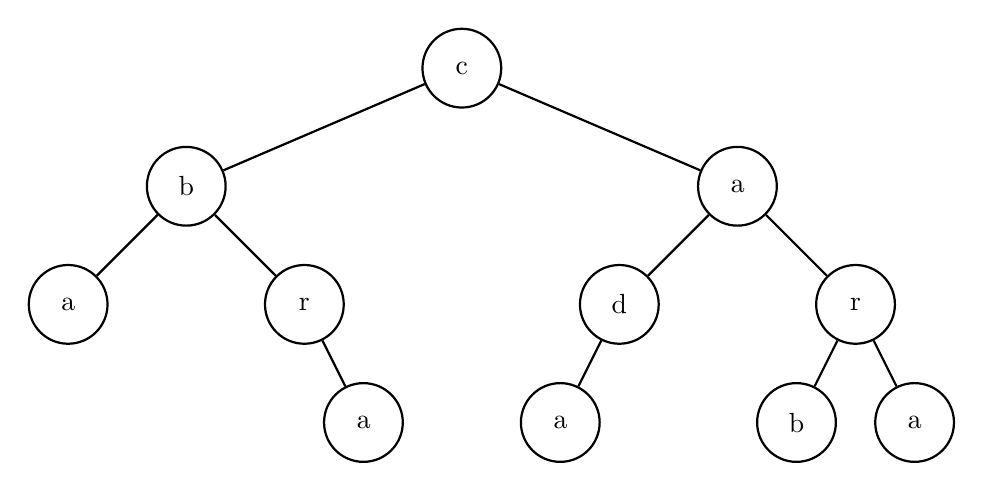
\begin{tikzpicture}[
                thick,
                every node/.style = {draw, circle, minimum size=10mm},
                level 1/.style = {sibling distance=70mm},
                level 2/.style = {sibling distance=30mm}, 
                level 3/.style = {sibling distance=15mm}, 
                level distance = 15mm
            ]
            \node {c}
                child {node {b}
                    child {node {a}}
                    child {node {r}
                        child[missing]
                        child {node {a}}
                    }
                }
                child {node {a}
                    child {node {d}
                        child {node {a}}
                        child[missing]
                    }
                    child {node {r}
                        child {node {b}}
                        child {node {a}}
                    }
                };
        \end{tikzpicture}
    \end{center}
\end{example}

Неявное ДДП не является обычным ДДП, т. к. тут нет того, что какой-то элемент меньше другого. Благодаря тому, что в поддереве поддерживается его размер, можно сделать, например, следующее:

\begin{itemize}
    \item Найти $k$-ый элемент по порядку
    \item Найти $k$-ый элемент по возрастанию
    \item Конкатенировать и разделять строки
    \item Добавлять/удалять элементы из любой позиции массива
\end{itemize}

\begin{note}
    Любое ДДП может быть по неявному ключу (AVL, красно-черное, B-дерево (хоть оно и не двоичное, но там аналогично)). $search(k)$ превращается в поиск $k$-того элемента, $insert(x, k)$ превращается во вставку в заданную позицию, а не по результатам сравнений (это делается с помощью размеров), $erase(k)$ теперь удаляет элемент на $k$-ой позиции.
\end{note}

\begin{definition}
    Операция $split$ получает на вход массив и число $k$. Задача в том, чтобы разбить массива на 2 массива, в первом из которых будет $k$ элементов, а во втором $n-k$, с сохранением порядка элементов.
\end{definition}

\begin{definition}
    Операция $merge$ получает на вход два массива ($m_1$ и $m_2$) и делает из них один массив ($m_1 + m_2$).
\end{definition}

\begin{note}
    Если реализовать эти две операции, то через них можно выразить и $insert$, и $erase$, и вообще все, что угодно.
\end{note}


\subsection{B-дерево \textcolor{red}{(-)}}


Пусть было 2 дерева. Слить их нереально, поэтому есть понятие ``слить 2 дерева и 1 ключ''. Свести слияние без ключа к слиянию с ключем можно без проблем (ключ очевидно должен быть больше всех вершин слева и меньше всех вершин справа). Пусть мы пока считаем, что глубины деревьев одинаковые. Тогда просто объединим эти 2 списка и эту 1 вершину, но если стало более чем $2t-1$ вершинки, то берем серединный ключ из списка и делаем его новым корнем. Заметим, что такое слияние работает за $O(1)$ (если считать $t$ константой). Теперь пусть у нас разные глубины. Глубины $h_1 < h_2$, и между ними есть еще 1 ключик. Тогда в левом дереве идем направо до тех пор, пока не дойдем до поддерева высоты $h_2$. Тогда просто объединяем эти 2 списка ключей (и тот доп ключик), если стало ключей больше чем $2t-1$, то опять разделяем и поднимаем какой-то из ключей наверх, и так поднимаемся. Получаем так называемый неоптимизированный аналог $insert$-а. Избежать подъема наверх нельзя, поэтому теперь все-таки придется хранить стек айдишников, чтобы понимать, кто у нас предок. Но, если мы идем сверху и гарантируем, что везде на пути (кроме вершины с которой мы мерджим) $< 2t - 1$ вершинок, то мы поднимемся наверх $O(1)$ раз, и сделаем $h_1 - h_2 + 2$ скачиваний (такое мы вроде умели делать в обычном $insert$-е), и асимптотика будет такой же. Кстати, можно не хранить глубину каждого поддерева, достаточно просто хранить глубину всего дерева. И еще, нам нужны размеры для неявности дерева, но их легко пересчитать без подъема наверх, т. к. мы знаем размер правого дерева, с которым мы сливаем. Это все очень круто, т. к. асимптотика зависит не от высоты, а от разности высот, поэтому если у нас очень глубокие деревья, но примерно с одинаковой глубиной, то все равно слияние будет довольно быстрым.

Попробуем теперь сделать сплит, но мы получаем не 2 массива, а массив длины $k-1$, $k$-тый элемент и еще массив длины $n - k$ (с сохранением порядка). Нам очень везет, если этот элемент находится в корне (пусть это элемент $C$). Если $C$ -- корень, то распиливаем список по элементу $C$, и вот мы и получили ответ (но надо еще пересчитать размер поддерева, для этого стоит хранить размеры всех детей). Если $C$ крайняя, то заметим, что нам не требуется возвращать 2 массива одинаковой глубины (и в интерфейсе даже ничего не сказано про глубину). Тогда просто разделим по этому элементу и вернем 2 дерева с разной глубиной. 

Теперь разберемся что делать, если $C$ не в корне. Пусть мы в корне и $C$ в каком-то поддерве. Отсплитим $2$ поддерва, и далее ``рекурсивно'' будем сплитить центральное поддерево. Если когда-то мы стоим с краю, то просто делаем дальше, только одной из частей (левой или правой) не будет. Когда-то мы придем в момент, когда мы попали в саму вершину $C$. Делаем финальный распил. Заметим, что нас попросили распилить на 2 поддерева, но мы немного перевыполнили план %[картинка дерева где было сделано дофигище сплитов пока не был найден нужный элемент]. 
Заметим, что деревья слева от вершинки $C$ имеют невозрастающие высоты (слева направо), а справа неубывающие (слева направо = убывающие справа налево). И заметим, что слева направо глубины деревьев строго убывают кроме первый двух. Но это пофиг - главное, что каждое следующие дереве не глубже предыдущего. Будем очевидно мерджить их по возрастанию высот, после мерджа высота будет либо $h$, либо $h + 1$, и т. к. высоты у деревьев отличаются не более чем на 1, то все сработает за очень быстро. %(отдельно тут докажем, что может быть не более 2-х деревьев подряд с одинаковой высотой (когда сплитим крайний элемент), и далее высота меньше ровно на 1).
Если высоты строго убывают, то при мердже правых деревьев у нас получается, что глубина слияния будет не более чем большее (левое) + 1, то есть не более чем дерево на 1 слева. Если же высоты могут быть одинаковыми, то может быть так, что было дерево высоты $h$, а правее него $h+1$, и обгон может быть и на много. Можно идти слева направо, храня все деревья в стеке, когда мы идем по деревьям и добавляем их в стек и видим, что последние 2 элемента равной глубины - то просто сливаем последние 2 и чекаем еще раз, после этого у нас будут строго убывающие глубины. Тогда асимптотика всех этих мерджей будет телескопической и в итоге будет $O(h)$, тогда удаление работает за $O(h)$.

Чтобы сделать реверс на подотрезке, надо развернуть массив и рекурсивно развернуть детей. Если сплит и мерж сверху, то теперь у нас разворот на подоотрезке не вероятностный, а честный.


\subsection{AVL-дерево \textcolor{red}{(-)}}


Давайте сливать тоже через 1 доп вершину. \\
Если есть 2 дерева одинаковой высоты и вершинка то можем слить за $O(1)$ (даже если они отличаются на $\pm 1$). Если $h_1 > h_2$, то идем в левом дереве направо, пока не дойдем до высоты $h_2$, удалим ребро в предка, и смерджим два дерева глубины $h_2$ и вершинку, и сделаем это все правым ребенком предка. %[картинка этого всего]. 
Если у какой-то вершины высота увеличилась на 1, то поворотами мы умеем решать эту проблему. Если рассмотреть все случаи то всегда все либо хорошо, либо очень легко решается поворотами (возможно мы даже раньше уже это решали). И все это работает за $O(h_1 - h_2)$.

Сплитим по $k$-му элементу. Если сплит по корню, то его отделяем и возвращаем его и его двух детей. Если нужно посплитить без ограничения общности в правом поддереве, то все оставляем и рекурсивно сплитим справа. %[картинка?]. 
Опять у нас как в B-дереве появляется цепочка деревьев, но в этот раз она может быть не невозрастающей. Посмотрим и подумаем, и заметим, что все-таки высоты невозрастают (если высота $h$ и справа брат имеет высоту $h+1$, то его левый ребенок имеет высоту $h$). Тогда как и в B-дереве мы умеем все это делать за $O(h)$


\subsection{Красно-черное дерево \textcolor{red}{(-)}}


Опять сливаем с доп. вершиной. Если у деревьев одинаковая черная глубина, тогда сделаем доп вершину черной и просто сделаем ее детей слева и справа. Если же разная черная глубина, опять слева спустимся до нужной черной глубины и просто как обычно все подвесим (справа), и сделаем доп вершину красной (чтобы не сломать черную глубину). Тогда сделаем доп вершину красной, и если у нас проблемы с красными вершинами, то как в инсерте просто решим эту проблему (т. к. у нас не более 1 раза когда у красной вершины красный ребенок, потому что справа черный корень, а слева мы можем выбрать вершину так, чтобы она была черной, поэтому проблема только с доп вершиной и ее предком).

Попробуем теперь сплитить. Делаем его как обычно -- если его номер меньше нужного, то слева будет левое поддерево и эта вершина, а справа рекурсивно сплитим. Если мы так будем делать, то опять черные высоты будут невозрастать, т. к. у любой вершины у ее детей одинаковые черные глубины. 
Если знак строгий и есть красные корни, то просто перекрашиваем корень в черный и неравенства получаются нестрогие. Но неравенства будут строгими, если корень был красным, так что все нормально мерджится и все круто.


Вывод: сплит и мердж это не только приколы декартача, но их можно делать вообще в любом дереве, причем иногда даже за честную асимптотику, а не за вероятностную.




\section{Задачи RSQ и RMQ}




Задачи RSQ (Range Sum Query) и RMQ (Range Minimum Query) мы теперь умеем решать с помощью split и merge в ДДПшках. \\
Static RSQ (массив не меняется) решается с помощью частичных (префиксных) сумм. \\
Static RMQ, в силу необратимости и идемпотентности операции $min$, решается с помощью Sparse Table (идея в том, что любой отрезок можно покрыть меньшими отрезками длины степени двойки, может быть с пересечением отрезков).


\subsection{Disjoined Sparse Table (продвинутый static RMQ)}


Решим продвинутую версию static RMQ. Пусть есть произвольная операция ЫТЬ: $A \times A \rightarrow A$. Дан массив из элементов $A$, он статичный, и про ЫТЬ известно только то, что она ассоциативна. Мы хотим отвечать на запрос ``ЫТЬ на подотрезке'' за $O(1)$, сделав $O(n log_2(n))$ предпосчета. Так как операция не обязана быть необратимой, то префиксные суммы использовать нельзя. Аналогично с идемпотентностью и спарсами. Для этого нам нужна новая структура данных.

Давайте построим что-то среднее между деревом отрезков и полным протоколом MergeSortа.

На каждом подотрезке из дерева отрезков давайте посчитаем префиксный и суффиксный ЫТЬ. На запрос отвечать будем следующим образом: если $L$ и $R$ с разных половин минимального отрезка, на котором они оба лежат, то берем в одном из более коротких отрезков суффиксный ЫТЬ, а в другом префиксный, и получаем ответ за $O(1)$. Если нет, то спустимся в ту половину, где они оба лежат, и продолжим рекурсивно, получаем ответ за $O(log_2(n))$. \\

Чтобы получать ответ за $O(1)$ нам нужно научиться быстро понимать, до какого уровня надо спускаться. Так как $n = 2^k$, то на первом уровне $L$ и $R$ будут в разных половинах тогда и только тогда, когда в их двоичной записи отличается старший бит, аналогично для любого $k$-го уровня и $k$-го бита соответственно. Тогда очевидно, что нам нужно найти самый старший бит, который отличается у границ отрезка, это легко сделать, взяв $L \oplus R$ (можно как в обычных спарсах предпосчитать логарифм (позицию старшей единицы) для всех чисел от 1 до $n$, а конкретный отрезок легко найти, т. к. зная уровень отрезка можно легко посчитать его длину).

\begin{note}
    Суммарная длина всех массивов равна $2n$. Если на каждом уровне записать подряд в один массив все суффиксные и префиксные ЫТЬ-и, то, поняв нужный уровень, мы можем просто взять $L$-ую ячейку суффикса и про-ЫТЬ-ить ее с $R$-ой ячейкой префикса.
\end{note}

\begin{note}
    В каждом отрезке можно считать либо только префиксные, либо только суффиксные ЫТЬ-и, причем они чередуются. Если так делать, то можно тратить в 2 раза меньше памяти, то есть столько же, сколько и в обычных спарсах. Это верно потому, что в двух соседних отрезках с одним родителем либо $L$ находится в левом, а $R$ в правом отрезке, либо это не так, и минимальный уровень, где $L$ и $R$ находятся в разных половинках от центра находится выше. 
\end{note}


\subsection{Дерево отрезков (Dynamic RSQ/RMQ)}


Храним мы его вот так (предполагая, что элементов $2^k$):
\begin{center} 
    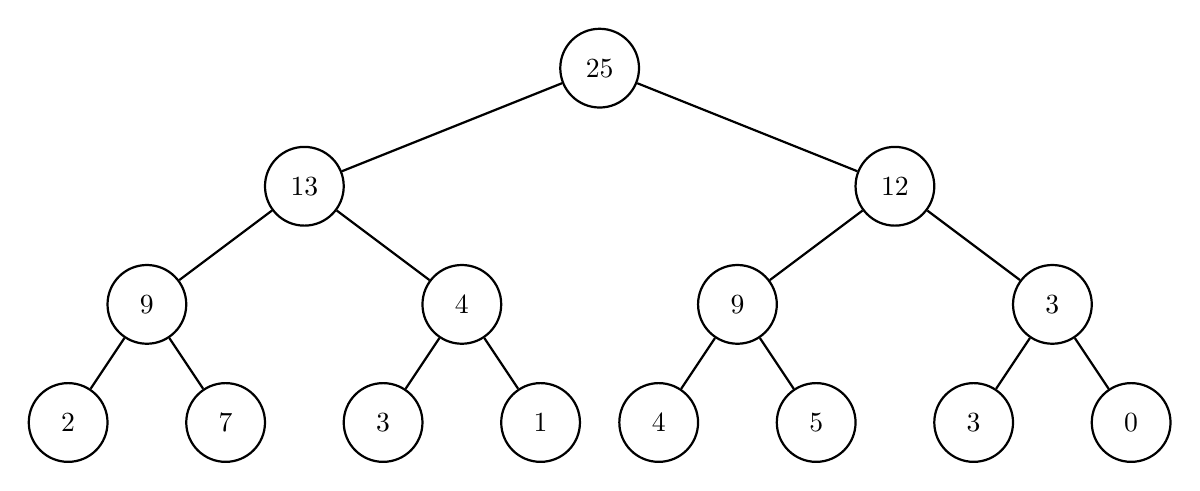
\begin{tikzpicture}[
            thick,
            every node/.style = {draw, circle, minimum size=10mm},
            level 1/.style = {sibling distance=75mm},
            level 2/.style = {sibling distance=40mm}, 
            level 3/.style = {sibling distance=20mm}, 
            level distance = 15mm
        ]
        \node {25}
            child {node {13}
                child {node {9}
                    child {node {2}}
                    child {node {7}}
                }
                child {node {4}
                    child {node {3}}
                    child {node {1}}
                }
            }
            child {node {12}
                child {node {9}
                    child {node {4}}
                    child {node {5}}
                }
                child {node {3}
                    child {node {3}}
                    child {node {0}}
                }
            };
    \end{tikzpicture}
\end{center}

В каждой ячейке сумма пересчитывается через 2 нижние. Если надо менять элемент в точке, то никакая рекурсия не нужна, просто меняем элемент и обновляем все сверху (прекрасно делается с помощью цикла while). Сумму можно тоже искать нерекурсивно: отрезок можно разбить на пары элементов с общим предком и не более двух ``лишних'' элементов (понимаем лишность элемента за $O(1)$). Убираем лишние, идем наверх и повторяем. Получаем ``ДО снизу'', код в котором получается красивее, чем в ДО сверху.